\documentclass[a4paper,twocolumn,12pt]{article}
\usepackage{url}
\usepackage{graphicx}
\usepackage{tikz-timing}

\title{gmZPU Wishbone Controller Datasheet}

\author{Koen Martens\\
        \texttt{kmartens@sonologic.nl}}

\begin{document}
\maketitle

\section{Introduction}

The gmZPU Wishbone Controller (ZWC) is a configurable WISHBONE B4 \cite{wishbone} compliant bus master. The ZWC connects to memory buses of a cpu as slave, and responds to read and write requests from the gmZPU. It supports classic WISHBONE B4 pipelined single cycles. Future revisions may support additional cycle types.


\section{Notation}

\begin{description}
    \item[BUS(1:0)] Bit 1 downto 0 of bus BUS.
\end{description}

\section{Overview}

The top design unit is \emph{zwishbone\_controller}. Figure \ref{fig:block_diagram} contains the conceptual block diagram of the \emph{ZWC}.

\begin{figure}[h]
    \centering
    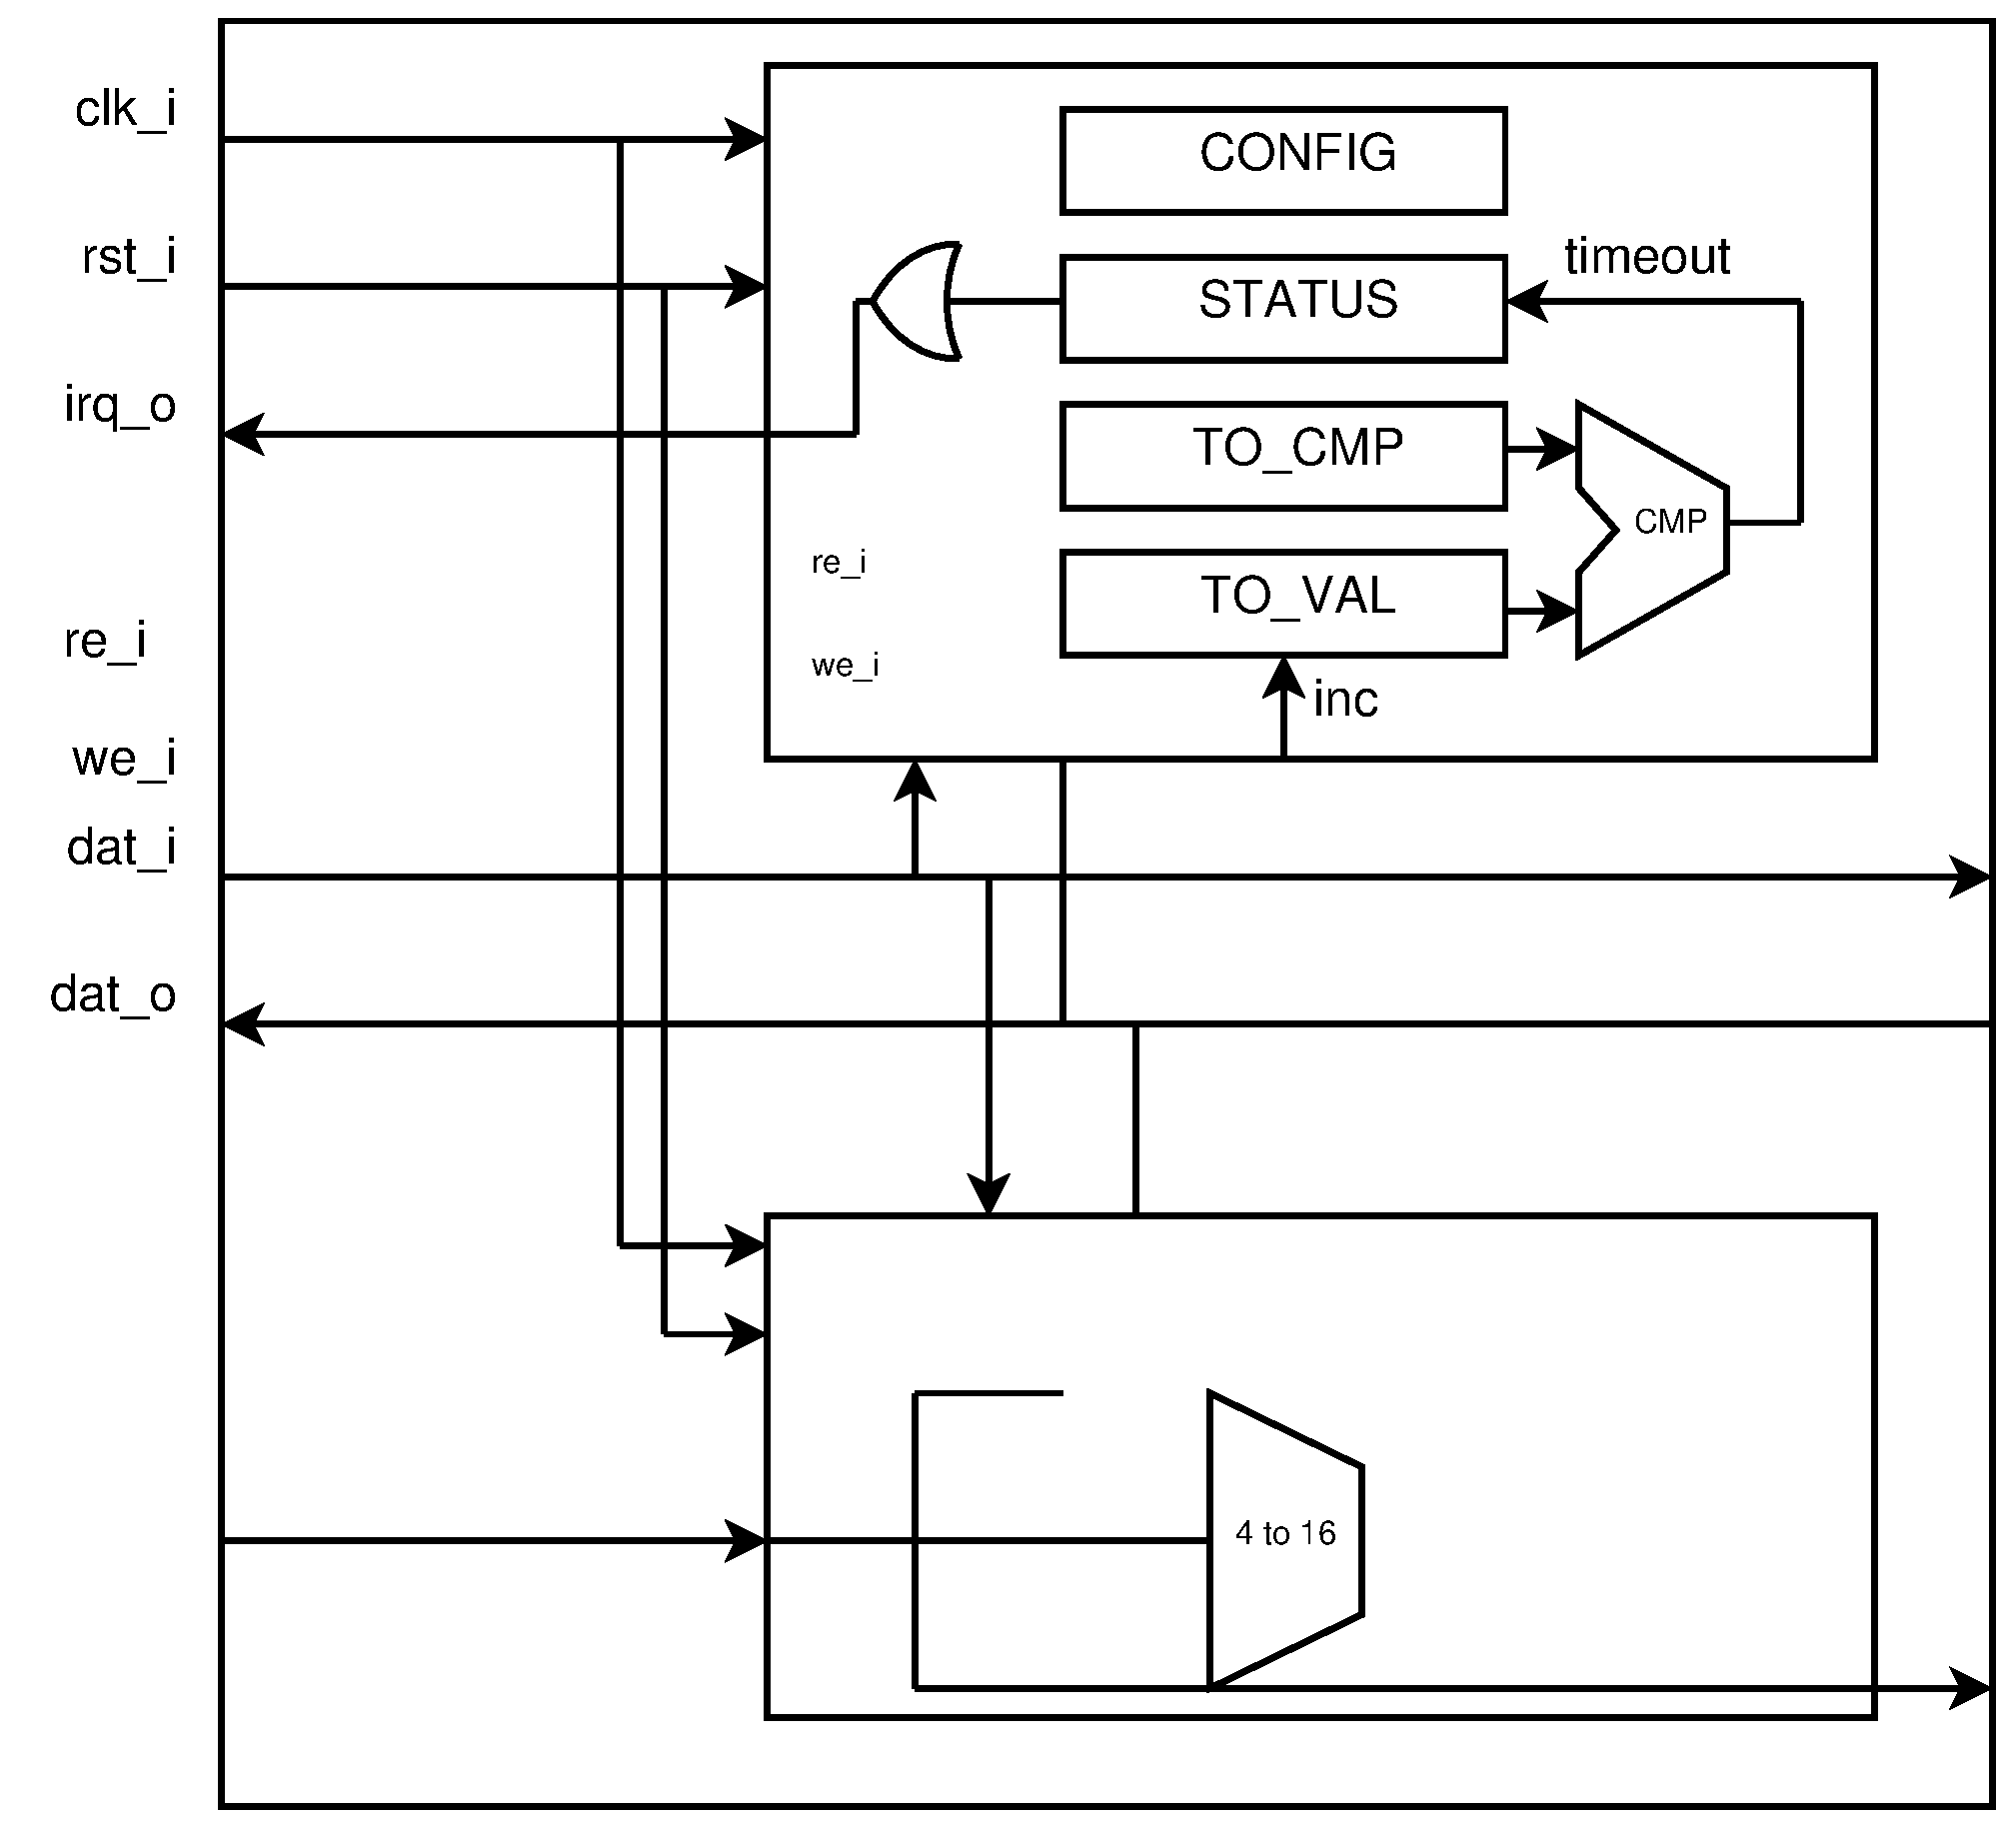
\includegraphics[width=7cm]{zwc_block_diagram}
    \caption{Block diagram}
    \label{fig:block_diagram}
\end{figure}

\subsection{Design constraints}

The \emph{ZWC} can have a variable address and data width. To comply with the WISHBONE B4 specification \cite{wishbone}, the data bus width must be 8, 16 or 32 bits.

The WISHBONE B4 \cite{wishbone} bus granularity is always equal to the data bus width.

The minimum address bus width configuration is shown in table \ref{tab:min_address}. Any additional bits added to the width of the address bus extend the WISHBONE B4 \cite{wishbone} address bus width.

\begin{table}[h]
\label{tab:min_address}
\begin{tabular}{| c | l | l |
}
    \hline
    bit & address(6)=0 & address(6)=1 \\ \hline \hline
    6 & 0 & 1 \\ \hline
    5 & reg\_addr(5) & chipselect(3) \\ \hline
    4 & reg\_addr(4) & chipselect(2) \\ \hline
    3 & reg\_addr(3) & chipselect(1) \\ \hline
    2 & reg\_addr(2) & chipselect(0) \\ \hline
    1 & reg\_addr(1) & bus\_addr(1) \\ \hline
    0 & reg\_addr(0) & bus\_addr(0) \\ \hline
\end{tabular}
\caption{Minimal address bus width configuration}
\end{table}

The MSB of the address bus decodes to the bus enable. If the bit is 1, the WISHBONE B4 \cite{wishbone} bus is selected. If the bit is 0, the controller registers are selected.

\section{Registers}

The CPU can control and check the operation of the ZWC by reading and writing to four registers:

\begin{description}
    \item[CONFIG] Controller configuration register
    \item[STATUS] Controller status register
    \item[TO\_CMP] Timeout counter compare value
    \item[TO\_VAL] Timeout counter value
\end{description}
\subsection{CONFIG}

The configuration register selects the WISHBONE B4 \cite{wishbone} bus cycle type. The bits in this register are defined in table \ref{tab:config_bits}. The current revision only supports pipelined cycles. All bits except PIPELINE (bit 0) of the CONFIG register should be written as 0. The result writing 1 to one of these bits is undefined.

\begin{table}[h]
\label{tab:config_bits}
\begin{tabular}{| c | c | c | c |
}
    \hline
    31 - 3 & 2 & 1 & 0 \\ \hline \hline
    reserved (write 0) & RMW & BLOCK & PIPELINE \\ \hline
\end{tabular}
\caption{CONFIG register bits}
\end{table}

\subsection{STATUS}

The STATUS register reflects the following error conditions:

\begin{description}
    \item[TO] Time out - a WISHBONE B4 cycle was initiated but the strobed slave did not respond
    \item[RTY] Retry - the WISHBONE B4 slave asserted wb\_retry
    \item[ERR] Error - the WISHBONE B4 slave asserted wb\_error
\end{description}

The bits in this register are defined in table \ref{tab:status_bits}.

\begin{table}[h]
\label{tab:status_bits}
\begin{tabular}{| c | c | c | c |
}
    \hline
    31 - 3 & 2 & 1 & 0 \\ \hline \hline
    reserved & TO & RTY & ERR \\ \hline
\end{tabular}
\caption{STATUS register bits}
\end{table}

\subsection{TO\_CMP}

The timeout compare register is compared with the TO\_VAL register. If the registers are equal, a timeout signal is asserted.

\subsection{TO\_VAL}

The timeout value register is an incrementing counter. It is reset to 0 at the start of a bus cycle. While the bus cycle is in progress, the register is incremented on each rising edge of the system clock.

The timeout value register is compared with the TO\_CMP register. If the registers are equal, a timeout signal is assertd. 

A timeout ends the bus cycle and sets the TO bit in the STATUS register. If the cycle was a read cycle, the value read by the cpu is undefined. If the cycle was a write cycle, no assumptions can be made about the current state of the slave. Specifically, no assumptions can be made regarding whether the value driven on the WISHBONE B4 bus was written to the destination within the slave or not.

\section{Timing}

This section contains timing diagrams.

\subsection{Register timing}

The CPU performs a register read in two cycles (see figure \ref{fig:reg_read_t}):

\begin{enumerate}
    \item On the first rising clock edge, the cpu drives the address bus and asserts \emph{re\_en}. The controller asserts \emph{busy}.
    \item On the second rising clock edge, the cpu releases the address bus and de-asserts \emph{re\_en}. The controller asserts \emph{ready} and drives the data bus.
\end{enumerate}

\begin{figure}[h]
        \begin{tikztimingtable}[
                xscale=2
            ]
            Clock    & 7{C}  \\
            re\_en   & L HH       LL        LL \\
            adr\_i   & U 2D{radr} UU        UU \\
            busy\_o  & L HH       LL        LL \\
            ready\_o & L LL       HH        LL \\
            dat\_o   & U UU       2D{value} UU \\
        \extracode
            \tablerules
            % Add vertical lines in two colors
            \begin{pgfonlayer}{background}
                \begin{scope}[semitransparent,semithick]
                    \vertlines[gray]{1,...,6}
                \end{scope}
            \end{pgfonlayer}
        \end{tikztimingtable}
    \caption{Register read timing}
    \label{fig:reg_read_t}
\end{figure}

The CPU performs a register write in one cycle, the register will be loaded on the second cycle (see figure \ref{fig:reg_write_t}):

\begin{enumerate}
    \item On the first rising clock edge, the cpu drives the address and data buses and asserts \emph{we\_en}. The controller prepares to latch the value on the data bus into the selected register.
    \item On the second rising clock edge, the cpu releases the address and data buses and de-asserts \emph{we\_en}. The controller latches the value into the selected register.
\end{enumerate}

\begin{figure}[h]
        \begin{tikztimingtable}[
                xscale=2
            ]
            Clock    & 7{C}  \\
            we\_en   & L HH       LL        LL \\
            adr\_i   & U 2D{radr} UU        UU \\
            busy\_o  & L LL       LL        LL \\
            ready\_o & L LL       LL        LL \\
            dat\_i   & U 2D{value} UU       UU \\
            register & U UU       4D{value}    \\
        \extracode
            \tablerules
            % Add vertical lines in two colors
            \begin{pgfonlayer}{background}
                \begin{scope}[semitransparent,semithick]
                    \vertlines[gray]{1,...,6}
                \end{scope}
            \end{pgfonlayer}
        \end{tikztimingtable}
    \caption{Register write timing}
    \label{fig:reg_write_t}
\end{figure}

\section{Application}

The reference design is the gmZPU \cite{gmzpu} System-on-Chip (SoC). The reference application of the design entity has a data width of 32 bits and an address width of 14 bits. A number of on-chip peripherals are connected to the gmZPU cpu by the ZWC.

\begin{thebibliography}{9}

\bibitem{wishbone} OpenCores \emph{Wishbone B4, WISHBONE System-on-Chip (SoC)Interconnection Architecture for Portable IP Cores} \url{http://opencores.org/opencores,wishbone} 2010.

\bibitem{gmzpu} Sonologic \emph{gmzpu github repository} \url{http://github.com/sonologic/gmzpu}.
\end{thebibliography}

\end{document}

